\documentclass[11pt,a4paper,sans]{moderncv}        % possible options include font size ('10pt', '11pt' and '12pt'), paper size ('a4paper', 'letterpaper', 'a5paper', 'legalpaper', 'executivepaper' and 'landscape') and font family ('sans' and 'roman')

%\usepackage{tikz,mwe}
\usepackage{tikz}
\newcommand{\tikzcircle}[2][, fill={rgb:black,2;white,2}]{\tikz[baseline=-0.7ex]\draw[#1,radius=#2] (2,0) circle ;}%
\usepackage{footmisc}

\newcommand*{\xingsocialsymbol}    {{\small\faXing}~} 
\newcommand*{\gitlabsocialsymbol}  {{\small\faGitlab}~} 
\newcommand*{\skypesocialsymbol}   {{\small\faSkype}~} 
\newcommand*{\stackoverflowsocialsymbol} {{\small\faStackOverflow}~}
\newcommand*{\bitbucketsocialsymbol} {{\small\faBitbucket}~}
\newcommand*{\orcidsocialsymbol} {{\small\faOrcid}~}
\newcommand*{\researchgatesocialsymbol}  {{\small\faResearchgate}~}
\newcommand*{\googlescholarsocialsymbol}  {{\small\faGoogleScholar}~}
\newcommand*{\telegramsocialsymbol}  {{\small\faTelegram}~}
\newcommand*{\whatsappsocialsymbol} {{\small\faWhatsapp}~}
\newcommand*{\bornsymbol} {{\small\faAsterisk}~}  

% moderncv themes
\moderncvstyle{classic
}          % style options are 'casual' (default), 'classic', 'oldstyle' and 'banking'
\moderncvcolor{blue}                                % color options 'blue' (default), 'orange', 'green', 'red', 'purple', 'grey' and 'black'
%\renewcommand{\familydefault}{\sfdefault}         % to set the default font; use '\sfdefault' for the default sans serif font, '\rmdefault' for the default roman one, or any tex font name
%\nopagenumbers{}                                  % uncomment to suppress automatic page numbering for CVs longer than one page

% character encoding
\usepackage[utf8]{inputenc}                       % if you are not using xelatex ou lualatex, replace by the encoding you are using
%\usepackage{CJKutf8}                              % if you need to use CJK to typeset your resume in Chinese, Japanese or Korean

% adjust the page margins
\usepackage[scale=0.75]{geometry}
%\setlength{\hintscolumnwidth}{3cm}                % if you want to change the width of the column with the dates
%\setlength{\makecvtitlenamewidth}{10cm}           % for the 'classic' style, if you want to force
%the width allocated to your name and avoid line breaks. be careful though, the length is normally
%calculated to avoid any overlap with your personal info; use this at your own typographical
%risks...

%Show labels in the bibliography
\makeatletter
\renewcommand*\bibliographyitemlabel{\@biblabel{\arabic{enumiv}}}
\makeatother
\renewcommand{\refname}{Last update: \today \vspace{2mm}}

\makeatletter
% commands from moderncvstylebanking.sty to have the title
% from that style
\newcommand*{\maketitlesymbol}{%
    {~~~{\rmfamily\textbullet}~~~}}% the \rmfamily is required to force Latin Modern fonts when using sans serif, as OMS/lmss/m/n is not defined and gets substituted by OMS/cmsy/m/n
%   internal command to add an element to the footer
%   it collects the elements in a temporary box, and checks when to flush the box
\newsavebox{\maketitlebox}%
\newsavebox{\maketitletempbox}%
\newlength{\maketitlewidth}%
\newlength{\maketitleboxwidth}%
\newif\if@firstmaketitleelement\@firstmaketitleelementtrue%
%   adds an element to the maketitle, separated by maketitlesymbol
%   usage: \addtomaketitle[maketitlesymbol]{element}
\newcommand*{\addtomaketitle}[2][\maketitlesymbol]{%
  \if@firstmaketitleelement%
    \savebox{\maketitletempbox}{\usebox{\maketitlebox}#2}%
  \else%
    \savebox{\maketitletempbox}{\usebox{\maketitlebox}#1#2}\fi%
  \settowidth{\maketitleboxwidth}{\usebox{\maketitletempbox}}%
  \ifnum\maketitleboxwidth<\maketitlewidth%
    \savebox{\maketitlebox}{\usebox{\maketitletempbox}}%
    \@firstmaketitleelementfalse%
  \else%
    \flushmaketitle{}\\%
    \savebox{\maketitlebox}{#2}%
    \savebox{\maketitletempbox}{#2}%
    \settowidth{\maketitleboxwidth}{\usebox{\maketitlebox}}%
    \@firstmaketitleelementfalse\fi}
%   internal command to flush the maketitle
\newcommand*{\flushmaketitle}{%
  \strut\usebox{\maketitlebox}%
  \savebox{\maketitlebox}{}%
  \savebox{\maketitletempbox}{}%
  \setlength{\maketitleboxwidth}{0pt}}
\renewcommand*{\maketitle}{%
  \setlength{\maketitlewidth}{0.8\textwidth}%
  \hfil%
  \parbox{\maketitlewidth}{%
    \centering%
    % name and title
    \namestyle{\@firstname~\@lastname}%
    \ifthenelse{\equal{\@title}{}}{}{\titlestyle{~|~\@title}}\\% \isundefined doesn't work on \@title, as LaTeX itself defines \@title (before it possibly gets redefined by \title) 
    % detailed information
    \addressfont\color{color2}%
    \ifthenelse{\isundefined{\@addressstreet}}{}{\addtomaketitle{\addresssymbol\@addressstreet}%
      \ifthenelse{\equal{\@addresscity}{}}{}{\addtomaketitle[~--~]{\@addresscity}}% if \addresstreet is defined, \addresscity and \addresscountry will always be defined but could be empty
      \ifthenelse{\equal{\@addresscountry}{}}{}{\addtomaketitle[~--~]{\@addresscountry}}%
      \flushmaketitle\@firstmaketitleelementtrue\\}%
    \collectionloop{phones}{% the key holds the phone type (=symbol command prefix), the item holds the number
      \addtomaketitle{\csname\collectionloopkey phonesymbol\endcsname\collectionloopitem}}%
    \ifthenelse{\isundefined{\@email}}{}{\addtomaketitle{\emailsymbol\emaillink{\@email}}}%
    \ifthenelse{\isundefined{\@homepage}}{}{\addtomaketitle{\homepagesymbol\httplink{\@homepage}}}%
    \collectionloop{socials}{% the key holds the social type (=symbol command prefix), the item holds the link
      \addtomaketitle{\csname\collectionloopkey socialsymbol\endcsname\collectionloopitem}}%
    \ifthenelse{\isundefined{\@extrainfo}}{}{\addtomaketitle{\@extrainfo}}%
    \flushmaketitle}\\[2.5em]}% need to force a \par after this to avoid weird spacing bug at the first section if no blank line is left after \maketitle

\renewcommand*{\namefont}{\Huge\bfseries\upshape}
\renewcommand*{\titlefont}{\Huge\mdseries\upshape}
\renewcommand*{\addressfont}{\normalsize\mdseries\upshape}
\renewcommand*{\quotefont}{\large\slshape}

% styles
\renewcommand*{\namestyle}[1]{{\namefont\textcolor{color1}{#1}}}
\renewcommand*{\titlestyle}[1]{{\titlefont\textcolor{color2!85}{#1}}}
\renewcommand*{\addressstyle}[1]{{\addressfont\textcolor{color1}{#1}}}
\renewcommand*{\quotestyle}[1]{{\quotefont\textcolor{color1}{#1}}}

\renewcommand*{\makecvtitle}{%
  % recompute lengths (in case we are switching from letter to resume, or vice versa)
  \recomputecvlengths%
  \maketitle%
  % optional quote
  \ifthenelse{\isundefined{\@quote}}%
    {}%
    {{\centering\begin{minipage}{\quotewidth}\centering\quotestyle{\@quote}\end{minipage}\\[2.5em]}}%
  \par}% to avoid weird spacing bug at the first section if no blank line is left after \maketitle}

\makeatother

% personal data
\name{Robert}{Krug}
\title{Curriculum Vitae}     
\extrainfo{Citizenship: Austrian \hspace{1mm} \tikzcircle{2pt} \hspace{1mm} Date of birth: $12/07/1981$}                 % optional, remove / comment the line if not wanted                          % optional, remove / comment the line if not wanted
\address{Faberstr. 8c}{81373 Munich}{Germany}% optional, remove / comment the line if not wanted; the "postcode city" and and "country" arguments can be omitted or provided empty
\phone[mobile]{+49 152 02407853}                   % optional, remove / comment the line if not wanted
\phone[fixed]{+49 711 811-92523}                    % optional, remove / comment the line if not wanted
\email{Robert.Krug4@de.bosch.com}                               % optional, remove / comment the line if not wanted
\social[linkedin][linkedin.com/in/robert-krug-74ab62164]{robert-krug}

%\homepage{www.kth.se/profile/rkrug?l=en}                         % optional, remove / comment the line if not wanted
\photo[64pt][0.4pt]{photo}                       % optional, remove / comment the line if not wanted; '64pt' is the height the picture must be resized to, 0.4pt is the thickness of the frame around it (put it to 0pt for no frame) and 'picture' is the name of the picture file
%\quote{Some quote}                                 % optional, remove / comment the line if not wanted

% to show numerical labels in the bibliography (default is to show no labels); only useful if you make citations in your resume
%\makeatletter
%\renewcommand*{\bibliographyitemlabel}{\@biblabel{\arabic{enumiv}}}
%\makeatother
%\renewcommand*{\bibliographyitemlabel}{[\arabic{enumiv}]}% CONSIDER REPLACING THE ABOVE BY THIS

% bibliography with mutiple entries
\usepackage{multibib}
\usepackage{enumitem}
\newcites{book,misc}{{Books},{Others}}
%----------------------------------------------------------------------------------
%            content
%----------------------------------------------------------------------------------
\begin{document}
%\begin{CJK*}{UTF8}{gbsn}                          % to typeset your resume in Chinese using CJK
%-----       resume       ---------------------------------------------------------
\makecvtitle

\newcommand\logocity[3][]{
  \tikz[baseline=(n.center)]
  \node(n)[align=center,inner sep=0,outer sep=0]{\includegraphics[#1]{#2}\\[1ex]#3};
}
\begin{picture}(0,0)
  \put(0,44){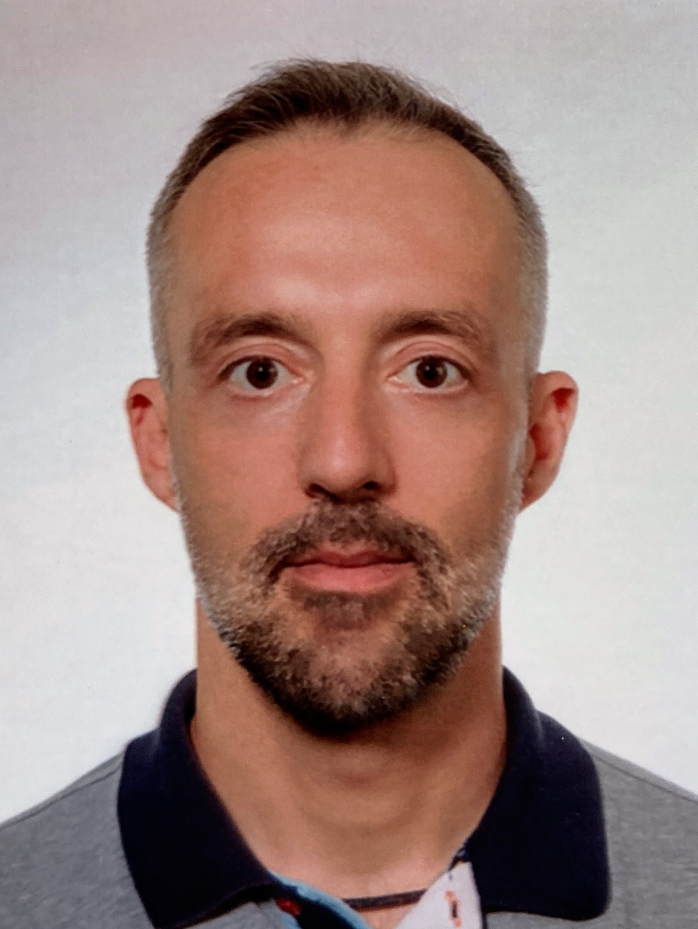
\includegraphics[scale=0.03]{photo.png}}
\end{picture}

\vspace{-5mm}
\section{Current Position}

\cventry{$2018$--present}{Research engineer}{}{}{R\&D Robotics, Robert Bosch GmbH, Stuttgart Area, Germany}{}
\begin{itemize}[leftmargin=1cm, itemsep=-2pt]
  \item Closed-loop multi-modal policy learning for industrial robot manipulation
  \item Reinforcement learning for robot manipulation tasks
  \item Model-based manipulator control with learned residuals
  \item Impedance-controlled insertion primitives for industrial robots

\end{itemize}
\section{Previous Positions}

\cventry{$2017$--$2018$}{Post-doctoral researcher}{}{}{Robotics, Perception and Learning lab,
  KTH Royal Institute of Technology, Stockholm, Sweden}{}

\cventry{$2014$--$2017$}{Post-doctoral researcher}{}{}{AASS Research Center,
  {\"O}rebro University, {\"O}rebro, Sweden}{}

\section{Education}
\cventry{$2009$--$2014$}{PhD in Control Theory}{}{}{AASS
  Research Center, {\"O}rebro University}{\textit{Thesis topic:} ``Optimization-based Robot Grasp
  Synthesis and Motion Control''.\\ \textit{Supervisors:} Prof. Achim J. Lilienthal and Dr. Dimitar
  N. Dimitrov.}

\cventry{$2001$--$2009$}{MSc in Mechatronics in Mechanical
  Engineering}{}{}{Graz University of Technology}{\textit{Thesis topic:} ``Dev. of a Flexible Handling- and Assemblysystem for Short Cycle
  Times''.\\ \textit{Supervisor:} Prof. Michael Hofbaur.}

\section{Teaching}

\cventry{$2018$}{Advanced Individual Course in Computer Science}{}{Masters level course}{KTH Stockholm}{Instructor}

\cventry{$2016$}{Robot Control\footnotemark}{}{Masters level course}{{\"O}rebro University}{Instructor}
%\footnotetext{Lecture notes available at:
%  \url{http://www.aass.oru.se/Research/Learning/rkg_dir/course_rc_2016.html}}

\cventry{$2011$}{Sensors and Sensing}{}{Masters level course}{{\"O}rebro University}{TA for Dr. Boyko Iliev}

\cventry{$2010$--$2011$}{Artificial Intelligence in Mobile Robots}{}{Masters level
  course}{{\"O}rebro University}{TA for Prof. Alessandro Saffiotti}

\cventry{$2005$--$2007$}{Principles of Dynamics}{}{Undergraduate course}{Graz University of
Technology}{TA for Prof. Andr\'{e}s Kecskem\'{e}thy \& Prof. Walter Sextro}

\cventry{$2005$--$2007$}{Principles of Statics}{}{Undergraduate course}{Graz University of
Technology}{TA for Prof. Andr\'{e}s Kecskem\'{e}thy \& Prof. Walter Sextro}

\section{Mentoring}

\cventry{}{Moritz Schneider}{}{Phd Co-Advisor}{R\&D Robotics, Robert Bosch GmbH}{}

\cventry{}{Sathiya Ramesh, Moritz Reuss, Sanjeev Kumar}{}{Masters Advisor}{R\&D Robotics, Robert Bosch GmbH}{}

\cventry{}{Shahbaz Kader, Michael Welle, Ioanna Mitsioni}{}{PhD Co-Advisor}{KTH Stockholm}{}

\cventry{}{Jens Lundell,  Jo\~ao Salvado}{}{PhD Co-Advisor}{{\"O}rebro University}{}

\cventry{}{Bowen Kuang, Dennis Malmgren, Alvin Sing Teck Lee}{}{Masters Advisor}{KTH Stockholm}{}

\cventry{}{Marcus A. Johansson, Chittaranjan Swaminathan}{}{Masters Advisor}{{\"O}rebro University}{}

\section{Research Grants and Projects}

\cventry{$2017$--$2020$}{FACT}{Factories of the Future: Human-robot Cooperative Systems}{Swedish Foundation for Strategic Research (SSF) project}{KTH Stockholm}{\textit{Role:} Scientific coordinator; co-advising PhD students.}

\cventry{$2017$--$2019$}{ROCOCO}{Multi-Timescale Robot Motion Planning and Control Using a Language of Constraints}{KKS ProSpekt project}{{\"O}rebro University}{\textit{Role:} Sole applicant (personal grant). \textbf{Grant returned due to change in position.}}

\cventry{$2017$--$2020$}{ILIAD}{Intra-Logistics with Integrated Automatic Deployment}{EU $H2020$
  project}{{\"O}rebro University}{\textit{Role:} Involved in proposal writing; co-advising PhD students.}

\cventry{$2017$--$2020$}{AMICI}{Augmented Interaction for Human-Robot Collaborative Tasks in
  Industrial Environments}{KKS H{\"O}G project}{{\"O}rebro University}{\textit{Role:} Involved in
  proposal writing; development of a whole-body controller for shared autonomy in telemanipulation.}

\cventry{$2016$--$2017$}{Re-LOAD}{Robot-aided Long-term Autonomous Drilling}{Vinnova pre-study
  grant}{{\"O}rebro University}{\textit{Role:} Involved in proposal writing; Overseeing the implementation and testing of force
  control schemes.}

\cventry{$2015$--$2019$}{AIR}{Action and Intention Recognition in Human Interaction with Autonomous
  Systems}{KKS SIDUS project}{{\"O}rebro University}{\textit{Role:} Contributing to robot intention
  communication via projection on shared floor space.}

\cventry{$2015$--$2018$}{SmokeBot}{Mobile Robots with Novel Environmental Sensors for Inspection of
  Disaster Sites with Low Visibility}{EU H$2020$ project}{{\"O}rebro University}{\textit{Role:} Integration of
  an optimization-based motion planning and control framework.}

\cventry{$2014$--$2015$}{APPLE}{Autonomous Picking and Palletizing}{Concept study project supported
  by KUKA}{{\"O}rebro University}{\textit{Role:} Involved in proposal writing; designing whole-body control schemes for
  simultaneous grasp planning and execution.}

\cventry{$2011$--$2015$}{RobLog}{Cognitive Robot for Automation of Logistic Processes}{EU FP$7$
  project}{{\"O}rebro University}{\textit{Role:} Responsible for grasp planning; development of
  compliant low-level grasp controllers.}

\cventry{$2009$--$2013$}{HANDLE}{Developmental Pathway towards Autonomy and Dexterity in Robot
  In-Hand Manipulation}{EU FP$7$ project}{{\"O}rebro University}{\textit{Role:} Learning of
  primitive grasp controllers; synthesis of grasp families from demonstrations.}

\section{Awards}
\cventry{$2015$}{KUKA Innovation Award Finalist}{}{}{}{Leading member of team APPLE - Autonomous
  Picking and Palletizing}

\cventry{$2013$}{Best Paper Finalist}{}{ICAR}{}{``Representing Movement Primitives as Implicit Dynamical Systems learned from Multiple Demonstrations''}

\section{Invited Talks}

\cventry{$2018$}{Planning, Learning and Controlling Robot Movement Behaviors}{}{Robert Bosch GmbH, Stuttgart Area}{}{}

\cventry{$2017$}{Planning as an Optimal Control Problem}{}{Lucia PhD School on ``Artificial Intelligence and Robotics'', ISR Lisbon}{}{}

\cventry{$2017$}{Integrated Perception and Control for Autonomous Manipulation}{}{MPI T{\"u}bingen}{}{}

\cventry{$2017$}{A Control Perspective on Robot Motion Behavior Generation}{}{KTH Stockholm}{}{}

\cventry{$2015$}{Grasp Envelopes for Constraint-based Robot Motion Planning and Control}{}{RSS -- Workshop on Bridging the Gap between Data-driven and Analytical Physics-based Grasping and Manipulation}{}{}

\cventry{$2012$}{Transfer of Grasp Families}{}{KTH Stockholm}{}{}

\section{Academic Activities}

\cventry{}{Reviewer}{}{ICRA, IROS, Humanoids, CASE, AAMAS, SAC, RAM, T-RO, T-ASE, AURO, RAS, RA-L, Advanced Robotics, Sensors}{}{}

\cventry{}{Workshop Organizer}{Closed-loop Grasping and Manipulation: Challenges and
  Progress}{}{IROS $2016$}{}

\cventry{}{Program Committee}{}{SAC $2017$, SAC $2016$}{}{}

\cventry{}{PhD Thesis Defense Committee}{Yuquan Wang}{KTH Stockholm}{$2016$}{}

\section{Publications}

An up-to-date publication list of peer-reviewed Conference and Journal papers as well as patents is available on Google Scholar\footnotemark.
\footnotetext{\url{https://scholar.google.se/citations?user=OZNzz9gAAAAJ\&hl=en}}
\vspace{4mm}
\nocite{*}
\bibliographystyle{IEEEtran}%plain,unsrt,alpha,abbrv,acm,apalike
\bibliography{Publications}

% \section{Languages}
% \cvitemwithcomment{German}{Native speaker}{}
% \cvitemwithcomment{English}{Proficient}{}
% \cvitemwithcomment{Swedish}{Basic}{}


% % Publications from a BibTeX file using the multibib package
% \section{Publications}
% \nocitebook{book1,book2}
% \bibliographystylebook{plain}
% \bibliographybook{publications}                   % 'publications' is the name of a BibTeX file
% \nocitemisc{misc1,misc2,misc3}
% \bibliographystylemisc{plain}
% \bibliographymisc{publications} 



\end{document}
